\documentclass[10pt]{article}
\usepackage{hyperref}
\usepackage{graphicx}
\usepackage[font=small,labelfont=bf]{caption}
\title{Biblioteca}
\author{carlo Sindico}
\begin{document}
\pagenumbering{arabic}



\begin{titlepage}

\newcommand{\HRule}{\rule{\linewidth}{0.5mm}} % Defines a new command for the horizontal lines, change thickness here

\center % Center everything on the page
 
%----------------------------------------------------------------------------------------
%	HEADING SECTIONS
%----------------------------------------------------------------------------------------

\textsc{\LARGE Universit\`a degli Studi di Padova}\\[1.5cm] % Name of your university/college
\textsc{\Large Laurea in Informatica}\\[0.5cm] % Major heading such as course name
\textsc{\large Corso di Programmazione ad Oggetti}\\[0.5cm] % Minor heading such as course title

%----------------------------------------------------------------------------------------
%	TITLE SECTION
%----------------------------------------------------------------------------------------

\HRule \\[0.4cm]
{ \huge  Progetto di fine corso}\\[0.3cm] % Title of your document
\HRule \\[1.5cm]
 
%----------------------------------------------------------------------------------------
%	AUTHOR SECTION
%----------------------------------------------------------------------------------------

\begin{minipage}{0.4\textwidth}
\begin{flushleft} \large
\emph{Studente:}\\
Carlo \textsc{Sindico} % Your name
\end{flushleft}
\end{minipage}
~
\begin{minipage}{0.4\textwidth}
\begin{flushright} \large
\emph{Matricola:} \\
\textsc{1069322} % Supervisor's Name
\end{flushright}
\end{minipage}\\[4cm]

% If you don't want a supervisor, uncomment the two lines below and remove the section above
%\Large \emph{Author:}\\
%John \textsc{Smith}\\[3cm] % Your name

%----------------------------------------------------------------------------------------
%	DATE SECTION
%----------------------------------------------------------------------------------------

{\large 3/02/2017}\\[3cm] % Date, change the \today to a set date if you want to be precise

%----------------------------------------------------------------------------------------
%	LOGO SECTION
%----------------------------------------------------------------------------------------

%\includegraphics{Logo}\\[1cm] % Include a department/university logo - this will require the graphicx package
 
%----------------------------------------------------------------------------------------

\vfill % Fill the rest of the page with whitespace

\end{titlepage}
\newpage
\pagenumbering{arabic}

\section{Ambiente di sviluppo}
\begin{itemize}
	\item Versione del compilatore: GCC 4.9.2 32bit
	\item Sistema opertivo utilizzato: Windows 10 (test funzionamento effettuati anche con Ubuntu 16.04LTS)
	\item Versione delle librerie Qt: 5.6.2 32bit
\end{itemize}
\section{Ore lavorative}
\begin{itemize}
	\item Sono state spese 35 ore per la parte relativa alla logica del progetto
	\item Sono state spese 25 ore per la parte relativa all'interfccia grafica, test e debugging
\end{itemize}

\section{Scopo del progetto}
\begin{itemize}
\item Il progetto ha lo scopo di fornire un semplice ed intuitivo sistema per l'amministrazione, attraverso una interfaccia grafica, di una biblioteca. La biblioteca contiene opere che sono caratterizzate da un titolo e da un identificativo univoco, ed ogni opera pu\'o essere di due tipi: libro o rivista.

\item Un libro \'e una particolare opera caratterizzata da un autore, mentre invece una rivista \'e caratterizzata da un anno di uscita.

\item Le opere della biblioteca possono venire prestate agli utenti, ogni opera contiene linformazione relativa al suo stato se essa disponibile al prestito e se presente nella biblioteca. Per quanto riguarda i libri non vi \'e alcun vincolo sul prestito, invece le riviste che hanno un anno di uscita superiore a 20 anni non possono essere prestate n\'e all\'utente basic n\'e all'utente pro.

\item La biblioteca fornisce unarea utente, attraverso la quale ogni utente pu prendere in prestito le opere. (possibilit di visualizzare le opere presenti nella biblioteca, e contemporaneamente quelle prese in prestito). Lutente attraverso questa interfaccia pu ricevere e restituire le opere.

\item Un utente caratterizzato da un nome, un cognome, un codice scale, un identi cativo univoco, una password e il numero di opere che ha in prestito.Un utente basic un particolare utente, caratterizzato da un nu-mero di opere che pu ricevere in prestito, ssato a 5. Un utente pro un particolare utente, caratterizzato da un numero di opere che pu ricevere in prestito, ssato a 8.

\item Andremo ad analizzare successivamente pi\'u in dettaglio la gerarchia opera.
\end{itemize}

\subsection{Funzionalit\'a disponibili all'amministratore}
\begin{itemize}
\item l'amministratore attraverso il sistema deve essere in grado di eseguire semplici azioni quali:
		\begin{enumerate}
		\item Visualizzare tutte le opere presenti nella biblioteca
		\item Visualizzare i dettagli di tutte le opere presenti nell'archivio, ed eventualmente di modificarne i parametri quali titolo autore o anno di uscita, a 					seconda che sia un libro o una rivista
		\item Visualizzare tutti gli utenti registrati alla biblioteca
		\item Visualizzare i dettagli di tutti gli utenti presenti nell'archivio, ed eventualmente di modificarne i parametri quali nome e cognome
		\item Aggiungere un'opera per aumentare l'offerta concessa dalla biblioteca
		\item Eseguire una ricerca di un'opera per titolo
		\item Eseguire una ricerca di un utente per nome
		\item Rimuovere un'opera 
		\item Aggiungere un utente all'archivio della biblioteca
		\item Rimuovere un utente solo se ha restituito tutte le opere prese in prestito
		\end{enumerate}
\end{itemize}

\subsection{Funzionalit\'a disponibili all'utente}
\begin{itemize}
\item l'utente attraverso il sistema deve essere in grado di eseguire semplici azioni quali:
		\begin{enumerate}
		\item Visualizzare tutte le opere presenti nella biblioteca
		\item Eseguire una ricerca di un'opera per titolo
		\item Ricevere in prestito secondo i limiti descritti precedentemente libri e riviste
		\item Restituire alla biblioteca libri e riviste
		\end{enumerate}
\end{itemize}

\section{Descrizione della gerarchia costituita da opera e dai suoi sottotipi}
\begin{itemize}

\begin{figure}[ht!]
\centering
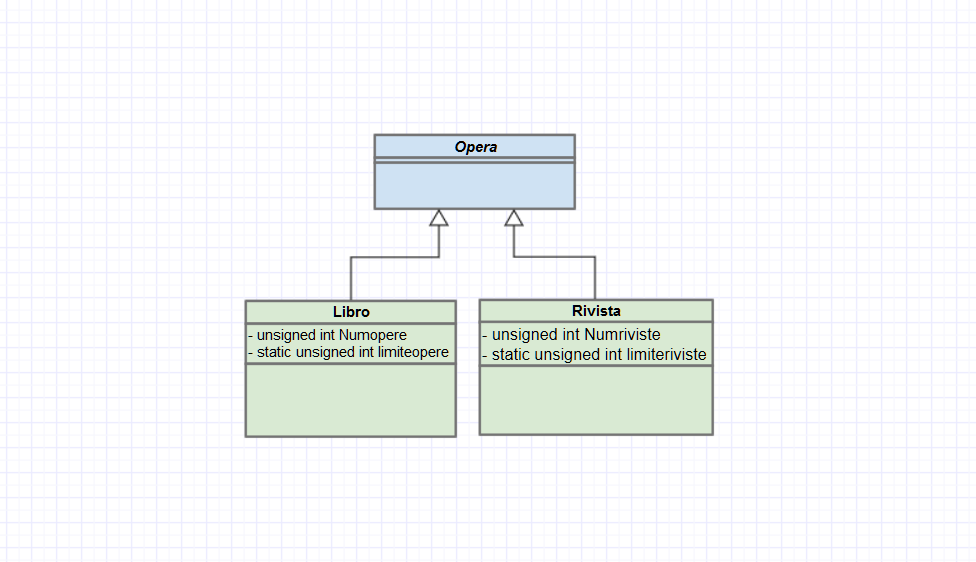
\includegraphics[scale=0.2]{opera}
\caption{vedi file opera.png}
\end{figure} 

\item \textbf{La classe opera alla base della gerarchia ed caratterizzata dai seguenti campi dati:}

		\item \underline{QString titolo}: titolo dellopera

		\item \underline{Bool statoPresenza}: indica se lopera presente nella biblioteca oppure in prestito, (1 indica la presenza dellopera nellarchivio) (0 			indica la non pre-senza ossia che in prestito).

		\item \underline{Int id}: identi cativo univoco dellopera, attribuito a ciascuna opera al mo-mento della costruzione dellopera stessa.

		\item \underline{Int maxid}: il massimo id dellopera, lopera con id pi elevato di tutte le altre e viene memorizzato in questa variabile.

		\item \underline{Int appartenenza}: variabile che indica a chi appartiene lopera (-1 valore attribuito quando lopera appartiene alla biblioteca) 			(idutente valore at-tribuito quando lopera appartiene ad un utente).

\item Inoltre sono presenti dei metodi non virtuali quali il costruttore:

		\item \underline{Opera(const QString\& , bool =0)}: costruttore a 1,2 argomenti che con-sente di costruire un'opera inserendo il solo titolo e 			segnalando di default che l'opera presente nella biblioteca; il corpo del costruttore consente di assegnare in automatico un ID univoco all'opera 				prendendo il massimo ID nora assegnato e facendo +1; in questo modo si assicura l'univocit degli ID.

\item Metodi get:

		\item \underline{QString GetTitolo()const}: metodo constante che consente di ritornare il titolo dell'opera.

		\item \underline{int Get Id() const}: metodo constante che consente di ritornare l'Id dell'opera.

		\item \underline{int Get MaxId() const}: metodo constante che consente di ritornare l'Id massimo assegnato ad un'opera no a questo momento.

\item Metodi di set:

		\item \underline{void Set Id(const int n) }: metodo che consente di modi care l'ID di un'opera
		facendolo diventare = n.

		\item \underline{void Set maxid(const int)}:  metodo che consente di aggiornare il campo dati maxId in modo che resti sempre il massimo Id 				assegnato ad un'opera.

		\item \underline{void Setappartenenza(const int)}: metodo che consente di aggiornare il campo dati appartenenza in modo che si ideni chi a chi 			appartiene quell'opera.

		\item \underline{int Getappartenenza() const}: metodo constante che consente di ritornare l'appartenenza di quell'opera.

		\item \underline{void Set Titolo(QString)}: metodo che consente di aggiornare il campo dati maxId in modo che resti sempre il massimo Id 				assegnato ad un'opera.

		\item \underline{void Riscatta()}: metodo che simula il ritorno in biblioteca di un'opera (set-tando statoP=1).

\item Metodi virtuali:

		\item \underline{virtual bool disponibile( )const}: metodo virtuale che ritorna true se l'opera di invocazione pu essere prestata, false altrimenti (in 		particolare questa una versione base che ritorna true se l'opera presente negli archivi della biblioteca).

		\item \underline{virtual void Write opera(QXmlStreamWriter\& xmlWriter) const =0} metodo che consente di scrivere nel le XML l'opera di 				invocazione. Esso puro in quanto Libro e Rivista hanno campi dati diversi.

		\item \underline{virtual void PrestaOpera()}: metodo che consente di prestare un'opera. stato scelto di segnarlo come virtuale in quanto vi sono 			delle regole diverse nei due sottotipi.

 		\item \underline{virtual info opera info tot() const =0}: metodo virtuale puro che consente di ritornare un oggetto di tipo info contenente tutte le 			informazioni relative all'opera di invocazione; il metodo virtuale puro in quanto le informazioni presenti nei sottotipi sono diverse.

		\item \underline{virtual QString Get tipo( ) const =0}: metodo virtuale puro che ritorna una stringa che rappresenta il tipo dell'opera di 					invocazione quindi se l'opera un libro il metodo ritorna la stringa libro mentre se una rivista ritorna rivista. (il metodo viene utilizzato solo in lettura)

\item \textbf{Classe libro:}

\item Metodi get:

		\item \underline{QString GetAutore() const}: metodo constante che consente di ritornare l'autore dell'opera

		\item \underline{void SetAutore(QString)}: metodo che consente di aggiornare il campo dati Autore di un libro.

\item Metodi virtuali:

		\item \underline{virtual void Write Opera(QXmlStreamWriter\& xmlWriter) const}: implementazione del metodo virtuale puro della classe base che consente la scrittura su database di un'opera.

		\item \underline{virtual info opera info tot( )const}: metodo che ritorna un oggetto di tipo info contenente tutte le informazioni riguardo all'oggetto di invocazione: titolo, autore, Id, prensenza in biblioteca e disponibilit al prestito.

		\item \underline{virtual QString Get tipo()const}: metodo che ritorna la stringa libro.

\item \textbf{Classe rivista:}

\item Metodi get:

		\item \underline{int GetMaxAnni( ) const}: metodo constante che consente di ritornare il numero massimo di anni entro il quale un'opera deve essere uscita per permettere il prestito.

		\item \underline{int GetAnnoUscita( ) const}: metodo constante che consente di ritornare l'anno di uscita della rivista di invocazione.

\item Metodi virtuali:

		\item \underline{virtual bool disponibile() const}: metodo che ritorna true se l'opera in bib-lioteca e se la sua data di uscita minore o uguale a maxAnni. Nel caso in cui ritorna true allora signi ca che l'opera pu venire prestata.

		\item \underline{virtual void Write opera(QXmlStreamWriter\& xmlWriter) const}: implemen-tazione del metodo virtuale puro della classe base che consente la scrittura su database di un'opera.

		\item \underline{virtual info opera info tot()const}: metodo che ritorna un oggetto di tipo info contenente tutte le informazioni riguardo all'oggetto di invocazione: titolo, anno di uscita, Id, prensenza in biblioteca e disponibilit al prestito

		\item \underline{virtual void PrestaOpera()}: metodo che testa la disponibilit della rivista di invocazione e presta l'opera se essa diponibile al prestito.

		\item \underline{virtual QString Get tipo()const}: metodo che ritorna la stringa rivista.
\end{itemize}


\section{Descrizione della gerarchia costituita da utente e dai suoi sottotipi:}
\begin{itemize}

\begin{figure}[ht!]
\centering
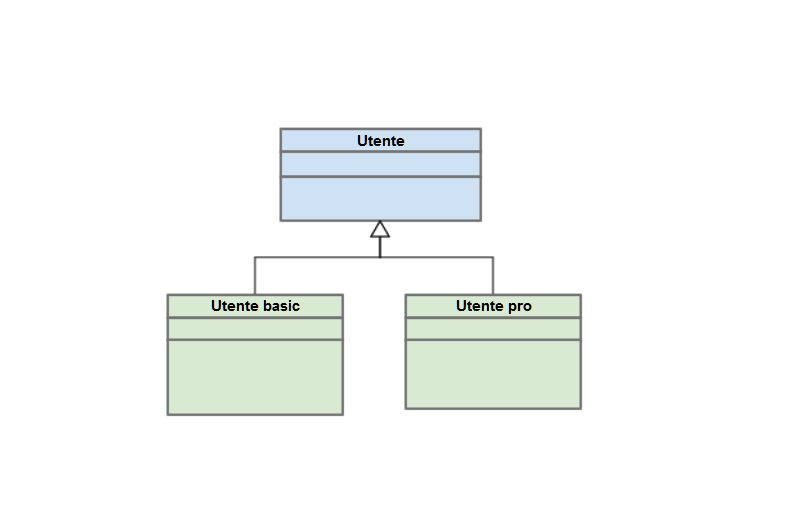
\includegraphics[scale=0.2]{utente}
\caption{vedi file utente.png}
\end{figure} 

 \item \textbf{La classe utente \'e alla base della gerarchia ed \'e caratterizzata dai seguenti metodi:}


		\item \underline{database utente opere* GetdbOpereUtente() const}: metodo che permette all'utente di interfacciarsi con il database delle sue opere.

		\item \underline{database* GetopereBiblioteca() const}: metodo che permette all'utente di interfacciarsi con database delle opere presenti nella biblioteca

		\item \underline{void ricevi libro() const=0}: metodo virtuale puro che permette all'utente di ricevere in prestito un libro, rispettando i limiti descritti precedentemente.

		\item \underline{void ricevi rivista() const=0}: metodo virtuale puro che permette all'utente di ricevere in prestito una rivista, rispettando i limiti descritti preceden-temente.

		\item \underline{void restituisci libro() const=0}: metodo virtuale puro che permette all'utente di restituire un libro.

		\item \underline{void restituisci rivista() const=0}: metodo virtuale puro che permette all'utente di restituire una rivista.

		\item \underline{bool checklimite() const=0}: metodo virtuale puro che restituisce true se l'utente abilitato a ricevere l'opera, false altrimenti.


\item	\textbf{Classe utente pro:}

 	\item nella classe utente pro vengono implementati tutti i metodi virtuali puri della classe base utente, rispettando il limite imposto ad un utente pro ossia limiteopere=8.

\item \textbf{Classe utente basic:}

\item nella classe utente pro vengono implementati tutti i metodi virtuali puri della classe base utente, rispettando il limite imposto ad un utente pro ossia limiteopere=5.

\end{itemize}


\section{Descrizione dell'interfaccia grafica}
\begin{figure}[ht!]
\centering
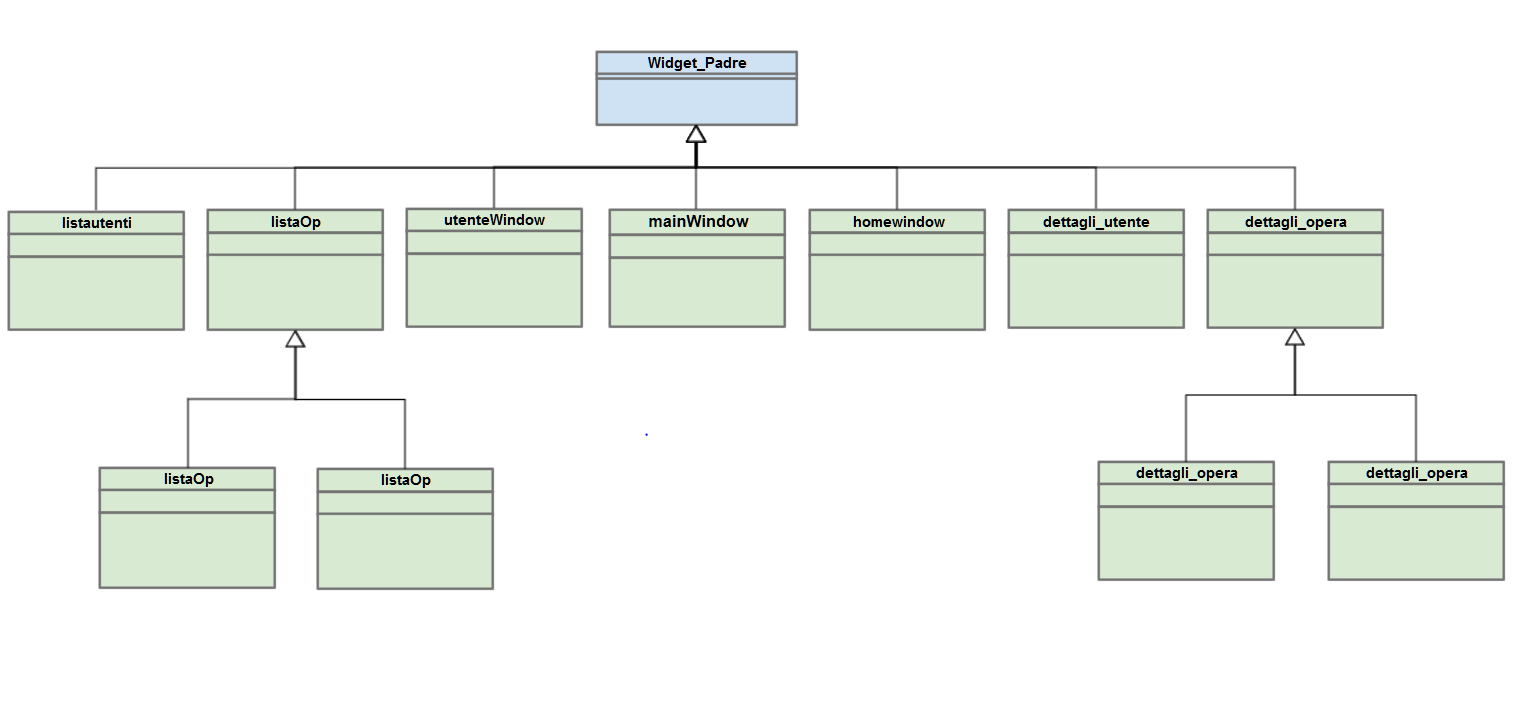
\includegraphics[scale=0.2]{view}
\caption{vedi file view.png}
\end{figure} 
\subsection{Descrizione della gerarchia costituita da Widgt padre e dei suoi sottotipi:}
\begin{itemize}
	\item Questa gerarchia \'e stata scelta per due motivi principali:

		\begin{enumerate}
		\item Tutte le view derivano da una base comune Widget padre, perci\'o in futuro sar\'a possibile aggiungere nuove funzionalit\'a al sistema, 				implementando altre view.
		\item Le view che derivano da Widget padre hanno delle caratteristiche in comune:
		\begin{itemize}
		\item Una MODEL di rifermiento rappresentata dalla classe database, databaseutente  e databaseutenteopere.
		\item I dati che vengono visualizzati nelle view vengono aggiornati in seguito ad azioni eseguite dall\'utente.
		\item Alle vie che vengono costruite, viene applicato uno stile.
		\end{itemize}
		\end{enumerate}

\item \textbf{Classe Widget padre:}


\item La classe Widget padre costituita \'e dai seguenti metodi:

		\item \underline{database* get model() const}: permette di accere al database delle opere presenti nella biblioteca.

		\item \underline{database utente* get modelutenti() const}: permette di accedere al database degli utenti registrati nella biblioteca.

		\item \underline{virtual void set style()}: metodo che permette di applicare lo stile alle view costruite.

		\item \underline{virtual void aggiorna vista( ) =0}: questo metodo permette di aggiornare
		i dati presenti nella vista di invocazione successivamente ad una azione dell'utente.

		\item \underline{virtual void costruisci contenuto( ) =0}: il metodo costruiscicontenuto per-mette di inserire per la prima volta i dati all'interno della view.

		\item \underline{void centra finestra( )}: questo metodo privato consente di centrare una nestra nel display al momento della creazione della stessa.
\end{itemize}

\subsection{Classe dettagli opera e lista opere:}
\begin{itemize}
\item La classe dettagli opera  \'e la classe base per 2 altre classi: dettagli rivista e dettagli libro. La scelta di inserire un'altra classe base \'e stata fatta in modo tale da favorire l'estensibilit del codice; in particolare nel caso in cui la biblioteca decida di gestire un' altra tipologia di opera ad esempio Documentario , il codice prevede gia una view base (lista opera) per visualizzare i dettagli della nuova opera redendo cosi facile l'inserimento di una nuova view con caratteristiche simili alle altre.
\end{itemize}
\end{document}
